\documentclass{beamer}
\usepackage{subcaption}
\usepackage{float}
\usepackage{setspace}
\usepackage{wrapfig}
\usepackage{caption}
\usepackage{mwe,tikz}\usepackage[percent]{overpic}
\captionsetup[figure]{labelformat=empty}
\usepackage{multirow}
\usepackage{array}
\newcolumntype{L}[1]{>{\raggedright\let\newline\\\arraybackslash\hspace{0pt}}m{#1}}
\newcolumntype{C}[1]{>{\centering\let\newline\\\arraybackslash\hspace{0pt}}m{#1}}
\newcolumntype{R}[1]{>{\raggedleft\let\newline\\\arraybackslash\hspace{0pt}}m{#1}}
\usetheme[pageofpages=of,% String used between the current page and the
                         % total page count.
          bullet=circle,% Use circles instead of squares for bullets.
          titleline=true,% Show a line below the frame title.
          alternativetitlepage=true,% Use the fancy title page.
          titlepagelogo=logo-polito,% Logo for the first page.
          watermark=watermark-polito,% Watermark used in every page.
          watermarkheight=100px,% Height of the watermark.
          watermarkheightmult=4,% The watermark image is 4 times bigger
                                % than watermarkheight.
          ]{Theme}
\usepackage{lmodern}
\author{\small By\\Bharat Bhushan (153100048)}
\title{{{Thermoelastic fracture problems using Extended Finite Element Method}}}
\institute{\small Under the guidance of\\Prof. Salil S. Kulkarni\\ \vspace{5pt}Department of Mechanical Engineering, IIT Bombay}
\date{\vspace{-5pt}October 18, 2016}
\begin{document}
%%%%%%%%%%%%%%%%%%%%%%%%%%%%%%%%%%%%%%%%%%%%%%%%%%%%%%%%%%%%%%%%%%%%5
%%%% TITLE PAGE %%%%%%%%%%%%%%%%%%%%%%%%%%%%%%%%%%%%%%%%%%%%%%%%%%%%
%%%%%%%%%%%%%%%%%%%%%%%%%%%%%%%%%%%%%%%%%%%%%%%%%%%%%%%%%%%%%%%%%%%%%
\begin{frame}[t,plain]
\titlepage
\end{frame}
%%%%%%%%%%%%%%%%%%%%%%%%%%%%%%%%%%%%%%%%%%%%%%%%%%%%%%%%%%%%%%%%%%%%%%
%%%% content %%%%%%%%%%%%%%%%%%%%%%%%%%%%%%%%%%%%%%%%%%%%%%%%%%%%%%%
%%%%%%%%%%%%%%%%%%%%%%%%%%%%%%%%%%%%%%%%%%%%%%%%%%%%%%%%%%%%%%%%%%%%

%%%%%%%%%%%%%%%%%%%%%%%%%%%%%%%%%%%%%%%%%%%%%%%%%%%%%%%%%%%%%%%%%
\begin{frame}[t,fragile]{Outline}
    \begin{itemize}
        \item Introduction  
        \item Motivation 
        \item Literature Survey 
        \item Work done 
        \item Problem definition 
        \item Conclusion 
    \end{itemize}
\end{frame}
%%%%%%%%%%%%%%%%%%%%%%%%%%%%%%%%%%%%%%%%%%%%%%%%%%%%%%%%%%%%%%%%%
\begin{frame}[t,fragile]{Introduction: Thermo-elastic Fracture Problems}
    \vspace{-.3cm}
    \begin{itemize}
        \item Due to heat transfer, temperature field is set up in the material which induces thermal stresses in the body.
\item These stresses becomes large in the vicinity of a discontinuity i.e. crack tip. If temperature variation is sufficiently large, it can lead to failure.
        \item Applications: Nuclear power plants, cylinder-nozzle
 intersection in pressure vessels, aerodynamic heating of high-speed aircraft, ultra fast pulse lasers etc.
   \end{itemize}
   \vspace{-.5cm}
\begin{figure}[H]
    \hspace{.7cm}
      \begin{subfigure}{0.45\textwidth}
    \centering
 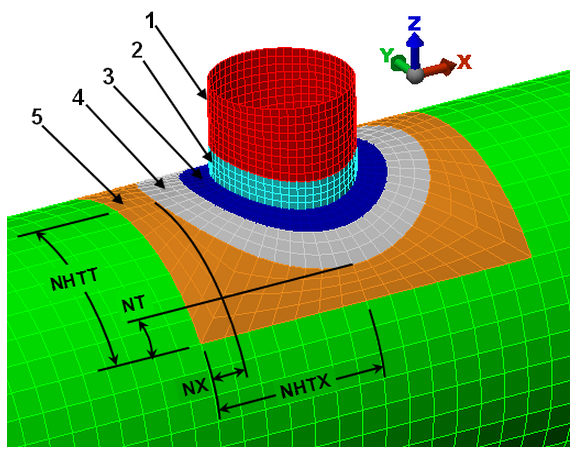
\includegraphics[scale=.1]{cyl.png}
 \caption{\tiny{The cylinder-nozzle intersection. (www.knowledge.autodesk.com)}}
 \label{cyl}
 \end{subfigure}
\begin{subfigure}{0.45\textwidth}
    \centering
 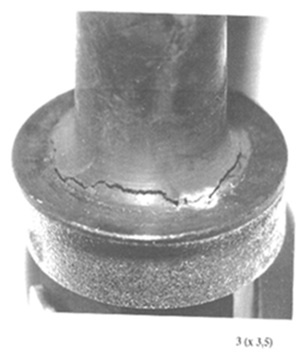
\includegraphics[scale=.1]{fail.jpg}
 \caption{\tiny{Cracked head of baffle bolt of Belgian Nuclear Reactor.(www.miningawareness.wordpress.com)}}
 \label{fail}
 \end{subfigure}
 \end{figure}
 \vspace{-.3cm}
   \tiny
   \hspace{15pt}
   \textbf{source}: Tian, X., Shen. (2006). A direct finite element method study of generalized thermoelastic problems. \\
   \vspace{-7pt}
   \hspace{15pt}
   \emph{International Journal of Solids and Structures}, 43(7), 2050-2063.
\end{frame}
%%%%%%%%%%%%%%%%%%%%%%%%%%%%%%%%%%%%%%%%%%%%%%%%%%%%%%%%%%%%%%%%%o 
\begin{frame}[t,fragile]{Why thermal load on crack is important?}
    \vspace{-.3cm}
    \footnotesize
\begin{itemize}
    \item Atkinson has solved the Dirichlet problem for Laplace's equation on a pie shaped region as $u(x,y)= r^{\frac{\pi}{\phi}}\sin\alpha\theta,\  r>0,\ 0<\theta<\phi$
        \begin{itemize}
                \footnotesize
    \item If $0<\phi<\pi$:
        The first partial derivative of u with respect to x and y remains continuous as we approach towards the origin. 
    \item If $\pi<\phi<2\pi$:
        The first derivative u with respect to x and y are not continuous as (x,y) approaches the origin. 
    \end{itemize}
    \item When $\phi=2\pi$, the problem becomes a crack problem and displacement and derivative of displacement vary as $u \propto r^{\frac{1}{2}}$ and $u'\propto  r^{-\frac{1}{2}}$ respectively. 
    \item As thermo-elastic problems are also governed by Laplace's equation, temperature will vary as $r^{\frac{1}{2}}$ and heat fluxes will be unbounded at the crack tip. 
\end{itemize}
  \tiny
  \vspace{10pt}
  \hspace{10pt}
   \textbf{source}: Atkinson, K. E. (1997).
    \emph{The numerical solution of \\
  \hspace{10pt}
    integral equations of the second kind} (Vol. 4). \\
  \hspace{10pt}
    Cambridge university press.
\begin{wrapfigure}{r}{0.4\textwidth}
    \centering
    \vspace{-50pt}
    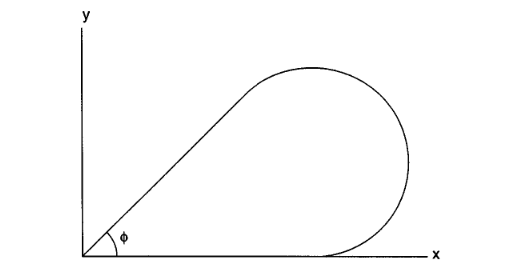
\includegraphics[width=.3\textwidth]{pie.png}
    \caption{\footnotesize Pie-shaped region.}
    \label{pie}
\end{wrapfigure}
 
\end{frame}
%%%%%%%%%%%%%%%%%%%%%%%%%%%%%%%%%%%%%%%%%%%%%%%%%%%%%%%%%%%%%%%%%%%%
\begin{frame}[t,fragile]{Finite Element Methods for Solving Thermoelastic Fracture Problems}
    \vspace{-.4cm}
    \begin{itemize}
        \item Methods for calculating stress intensity factors in FEM can be divided in two categories,
            \begin{itemize}
                \item Substitution method 
                \item Energy method 
            \end{itemize}
        \item In substitution method, we can get the SIF's as:
            \footnotesize
            $$ u=\frac{1+\nu}{4E}\sqrt{\frac{2r}{\pi}}\left\{ K_I\left[ (2\kappa -1)\cos \frac{\theta}{2}-\cos \frac{3\theta}{2} \right]+K_{II}\left[ (2\kappa +3)\sin\frac{\theta}{2}+\sin\frac{3\theta}{2} \right] \right\}$$
            \normalsize
A similar equation exist for $v$ also. 
        \item Using energy method, SIF's can be calculated as$^\ast$ 
            \footnotesize
$$G=-\frac{d\Pi}{da}\ ,\ \ \ \ \ \  
\Pi=-\frac{1}{2}{u}^T[K]{u}+\frac{1}{2}\int{\varepsilon_0}^T[D]{\varepsilon_0}dV$$
 
    \end{itemize}
    \vspace{-.1cm}
   \tiny
   \hspace{15pt}
   $^\ast$\textbf{source}:Hellen, T. K., \& Cesari, F. (1979). On the solution of the centre cracked plate with a quadratic thermal\\ 
   \vspace{-7pt}
   \hspace{15pt}
   gradient.\emph{Engineering Fracture Mechanics}, 12(4), 469-478.
\end{frame} 
%%%%%%%%%%%%%%%%%%%%%%%%%%%%%%%%%%%%%%%%%%%%%%%%%%%%%%%%%%%%%%%%%%%
\begin{frame}[t,fragile]{Extended Finite Element Method in Thermoelasticity}
    \begin{itemize}
        \item We have to use very fine mesh at capture the behaviour of crack.
\item In XFEM, we enrich the polynomial approximation to include the effects of singular discontinuous field.
    \item Advantages:
    \begin{itemize}
        \item Mesh is prepared without considering the existence of discontinuity.
        \item No need of remeshing.
    \end{itemize}
\end{itemize}
\begin{figure}
     \centering
     \vspace{-10pt}
     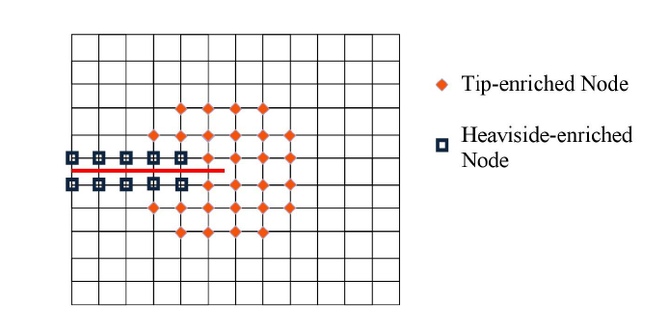
\includegraphics[scale=.3]{enrich.png}
     \caption{\hspace{-2cm}\footnotesize XFEM enrichment strategy}
  \end{figure}
\end{frame}
%%%%%%%%%%%%%%%%%%%%%%%%%%%%%%%%%%%%%%%%%%%%%%%%%%%%%%%%%%%%%%%%%%%%%%%%%%%%
%%%%%%%%%%%%%%%%%%%%%%%%%%%%%%%%%%%%%%%%%%%%%%%%%%%%%%%%%%%%%%%%%%%%%%%%%%%%
\begin{frame}[t,fragile]{Two types of enrichment functions in XFEM}
    \vspace{-.3cm}
     \footnotesize
    \begin{itemize}
        \item The nodes which belongs to the elements totally cut by the crack, are enriched by and Heaviside function.
    $$h(x,y)=\begin{cases}1,&       for ~ ~ y\ge 0\\ -1,&       for~ ~ y\le 0\end{cases}$$
\item The nodes of elements which contains cracktip are enriched by $\gamma$:
     \footnotesize
    \begin{align*}
    u^h&=\sum_i N_i(x)u_i+\sum_{j\in J} N_j(x) h(x)a_j+\sum_{k\in K} N_k(x)\left( \sum_{l=1}^{4}\gamma_l(x)b_{kl} \right) \\
    v^h&=\sum_i N_i(x)v_i+\sum_{j\in J} N_j(x) h(x)c_j+\sum_{k\in K} N_k(x)\left( \sum_{l=1}^{4}\gamma_l(x)d_{kl} \right) \\ 
    where,\ \ \ \gamma&=\left[ \sqrt{r}\cos \left( \frac{\theta}{2} \right), \sqrt{r}\sin\left( \frac{\theta}{2} \right),\sqrt{r}\sin\left( \frac{\theta}{2} \right)\sin(\theta),\sqrt{r}\cos\left( \frac{\theta}{2} \right)\sin(\theta)\right] 
\end{align*}
\end{itemize}
\tiny
\hspace{10pt}
\textbf{Source:}Belytschko, T., \& Black, T. (1999). Elastic crack growth in finite elements with minimal remeshing. \\
\vspace{-7pt}
\hspace{10pt}
\emph{International journal for numerical methods in engineering}, 45(5), 601-620.
\end{frame}
%%%%%%%%%%%%%%%%%%%%%%%%%%%%%%%%%%%%%%%%%%%%%%%%%%%%%%%%%%%%%%%%%%%%%%%%
\begin{frame}[t,fragile]{Which Nodes to Enrich? - Level Set Method}
    \vspace{-.3cm}
    \footnotesize
    \begin{itemize}
        \item There are two level-set functions defined as follows:
          \begin{itemize}
        \item Normal level set, $\psi(x)=$ the signed distance from the crack surface.
        \item Tangent level set, $\phi(x)=$ the signed distance to the plane including the crack front and perpendicular to the crack surface.
        \end{itemize}
    \item To decide which enrichment should be used. 
        \begin{itemize}
            \item If $\phi < 0 $ and $\psi_{min}\psi_{max}\leq 0$, nodes should be enriched with $h(x)$.
            \item If $\phi_{min}\phi_{max}\leq 0$ and $\psi_{min}\psi_{max}\leq 0 $, nodes should be enriched with $\gamma$.
        \end{itemize}
    \end{itemize}
  \begin{figure}
                \centering
                \vspace{-15pt}
                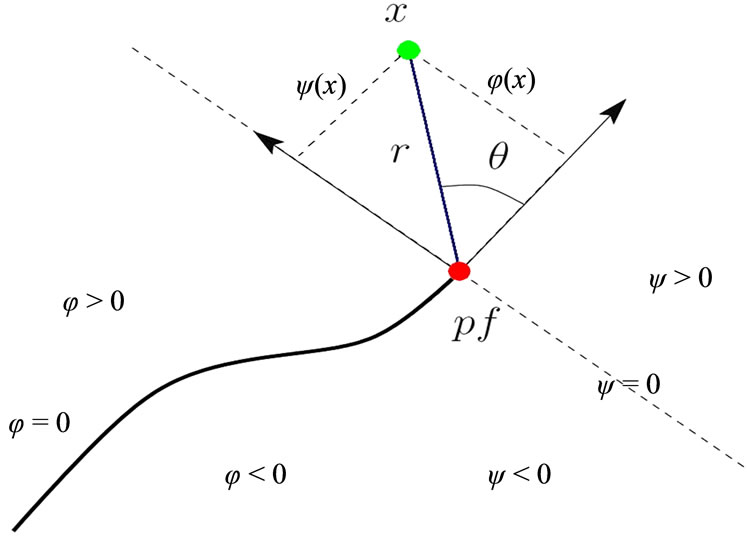
\includegraphics[scale=.15]{levelset.jpg}
                \caption{\tiny Level Set Method}
                \label{4}
            \end{figure}
    \tiny 
    \vspace{-20pt}
  \hspace{10pt}
    \textbf{Source:} Abdelaziz, Y., Bendahane, K., \& Baraka, A. (2011). Extended Finite Element Modeling: Basic Review and\\
  \vspace{-1pt}
  \hspace{10pt}
    Programming. Engineering, 3(07), 713.

\end{frame}
%%%%%%%%%%%%%%%%%%%%%%%%%%%%%%%%%%%%%%%%%%%%%%%%%%%%%%%%%%%%%%%%%%%%%%%%%%%%%%%
\begin{frame}[t,fragile]{Work Done}
    \begin{itemize}
        \item Finite Element Formulation of coupled thermoelasticity 
        \item Development of a MATLAB program for semi-coupled thermoelastic problems.
        \item Patch tests to validate the developed FEM program.
        \item Solution of various thermoelastic fracture problems and comparison with the analytical solutions. 
        \item Comparison between the solutions of FEM and XFEM programs. 
    \end{itemize}
\end{frame}
%%%%%%%%%%%%%%%%%%%%%%%%%%%%%%%%%%%%%%%%%%%%%%%%%%%%%%%%%%%%%%%%%%%
\begin{frame}[t,fragile]{Finite Element Formulation of Thermo-elasticity}
\begin{itemize}
\item We will formulate the semi-coupled in which we neglect the effect of displacements on temperature field.
\item In thermoelastic case the total strain is given as: 
\begin{align*}
    \varepsilon_{ij}&=\varepsilon_{ij}^{(M)}+\varepsilon_{ij}^{(T)}
    =\frac{1+\nu}{E}\sigma_{ij}-\frac{\nu}{E}\sigma_{kk}\delta_{ij}+\alpha(T-T_0)\delta_{ij}\nonumber
\end{align*}
\item Which can be inverted to get following stress-strain relationship:
    \footnotesize
\begin{align*}
    \begin{Bmatrix}
        \sigma_{x}\\ \sigma_{y}\\ \tau_{xy} 
    \end{Bmatrix} =\frac{E}{(1-\nu^2)}
    \begin{bmatrix}
        1 & \nu & 0 \\ \nu & 1 & 0 \\ 0 & 0 & 1-\nu 
    \end{bmatrix}
    \begin{Bmatrix}
        \varepsilon_{x}-\alpha\Delta T \\ \varepsilon_{y}-\alpha \Delta T \\ \varepsilon_{xy} 
    \end{Bmatrix}
\end{align*}
\end{itemize}

\end{frame}
%%%%%%%%%%%%%%%%%%%%%%%%%%%%%%%%%%%%%%%%%%%%%%%%%%%%%%%%%%%%%%%
   \begin{frame}[t,fragile]{Governing Equations of Thermoelasticity}
    \begin{itemize}
        \item The governing equations of the thermo-elasticity is derived as: 
            \bgroup
            \footnotesize
            \begin{align*}
    \frac{\partial}{\partial x}\left[c_{11}\frac{\partial u}{\partial x}+c_{12}\frac{\partial v}{\partial y}\right]+&\frac{\partial}{\partial y}\left[c_{66}\left(\frac{\partial u}{\partial y}+\frac{\partial v}{\partial x}\right)\right]-(c_{11}+c_{12})\alpha\frac{\partial T}{\partial x}-f_x   =0 \\
    \frac{\partial}{\partial x}\left[c_{66}\left(\frac{\partial u}{\partial y}+\frac{\partial v}{\partial x}\right)\right]+&\frac{\partial}{\partial y}\left[c_{12}\frac{\partial u}{\partial x}+c_{22}\frac{\partial v}{\partial y}\right]-(c_{11}+c_{12})\alpha\frac{\partial T}{\partial y}-f_y=0\\
    &\ \ \ \ \ \ \ k\left( \frac{\partial^2 T}{\partial x^2}+\frac{\partial^2 T}{\partial y^2} \right)=q
\end{align*}
\egroup
      \item We can develop a week form of above equations by approximating u,v and T over a typical finite element $\Omega^e$ as:
          \footnotesize
\begin{align*}
    u(x,y)=\sum_{i=1}^nN_i (x,y)u_i\ \ , 
    v(x,y)=\sum_{i=1}^nN_i (x,y)v_i\ \ ,
    T(x,y)=\sum_{i=1}^nN_i (x,y)T_i
\end{align*}
\end{itemize}
\end{frame}
%%%%%%%%%%%%%%%%%%%%%%%%%%%%%%%%%%%%%%%%%%%%%%%%%%%%%%%%%%%%%%%%%%%%%%
\begin{frame}[t,fragile]{Weak Form Equations of Coupled Thermoelasticity}
    \vspace{-.4cm}
            \scriptsize
        \begin{align*}
     -\int_{\Omega}^{}\left[ c_{11}\frac{\partial N_i}{\partial x}\frac{\partial N_j}{\partial x}u_j+c_{12}\frac{\partial N_i}{\partial x}\frac{\partial N_j}{\partial y}v_j\right]dxdy+\int_{\Omega}^{}\left[c_{66}\frac{\partial N_i}{\partial y}\frac{\partial N_j}{\partial y}u_jdxdy+\frac{\partial N_i}{\partial y}\frac{\partial N_j}{\partial x}v_j\right]dxdy\nonumber\\ -\int_{\Omega}^{}\frac{\partial N_i}{\partial x}\beta N_jT_j dxdy +\int_{\Omega}^{}N_if_x
     dxdy+\int_{\Gamma}^{}N_i\vec{t}dx=0\end{align*}
 \begin{align*}
     -\int_{\Omega}^{}\left[ c_{11}\frac{\partial N_i}{\partial y}\frac{\partial N_j}{\partial y}v_j+c_{12}\frac{\partial N_i}{\partial y}\frac{\partial N_j}{\partial x}u_j\right]dxdy+\int_{\Omega}^{}\left[c_{66}\frac{\partial N_i}{\partial x}\frac{\partial N_j}{\partial x}v_jdxdy+\frac{\partial N_i}{\partial x}\frac{\partial N_j}{\partial y}u_j\right]dxdy\nonumber\\ -\int_{\Omega}^{}\frac{\partial N_i}{\partial y}\beta N_jT_j dxdy+\int_{\Omega}^{}N_if_y dxdy+\int_{\Gamma}^{}N_i\vec{t}dy=0
 \end{align*}
 \begin{align*}
        k\int_{\Omega}\left( \frac{\partial N_i}{\partial x}\frac{\partial N_j}{\partial x}+\frac{\partial N_i}{\partial y}\frac{\partial N_j}{\partial y} \right)T_jdxdy-\int_{\Omega}^{}N_iN_jqdxdy=\int_{\Gamma}^{}N_i\bar{Q}ds& \end{align*}
\end{frame}
%%%%%%%%%%%%%%%%%%%%%%%%%%%%%%%%%%%%%%%%%%%%%%%%%%%%%%%%%%%%%%%%%%%
\begin{frame}[t,fragile]{Finite Element Model}
    \vspace{-.3cm}
    \footnotesize
    \begin{itemize}
        \item Neglecting the body forces, above equations can be written in matrix form as: 
    \begin{align*}
\begin{bmatrix}
    K_{11} & K_{12} \\
    0 & K_{22}
\end{bmatrix}
\begin{Bmatrix}
    U^e\\ T^e
\end{Bmatrix}=
\begin{Bmatrix}
    F\\ Q
\end{Bmatrix}
\end{align*}
Where,
\vspace{-.2cm}
    \scriptsize
\begin{align*}
    [K_{11}^e]=\int_{\Omega}[B]^T[C][B]dxdy\ \
    [K_{12}^e]=\int_{\Omega}[B]^T[\beta][N^{\theta}]dxdy\ \
    [K_{22}^e]=\int_{\Omega}[B^{\theta}]^T[K][B^{\theta}]dxdy
\end{align*}
\vspace{-.5cm}
\begin{align*}
    \{F\}=\int_\Gamma [N]^T{\bar{t}}ds\ \
    \{Q\}=\int_\Gamma [N^{\theta}]^T\bar{Q}ds
\end{align*} 
\vspace{-.5cm}
\end{itemize}
    \scriptsize
\begin{align*}
    [B]=\begin{bmatrix}
        \frac{\partial N_1}{\partial x}&0&\frac{\partial N_2}{\partial x}&0&\dots&\frac{\partial N_n}{\partial x}&0\\
        0&\frac{\partial N_1}{\partial y}&0&\frac{\partial N_2}{\partial y}&\dots&0&\frac{\partial N_n}{\partial y}\\
\frac{\partial N_1}{\partial y}&\frac{\partial N_1}{\partial x}&
\frac{\partial N_2}{\partial y}&\frac{\partial N_2}{\partial x}&\dots&
\frac{\partial N_n}{\partial y}&\frac{\partial N_n}{\partial x}
    \end{bmatrix},\   [B^{\theta}]=\begin{bmatrix}
        \frac{\partial N_1}{\partial x}&\frac{\partial N_2}{\partial x}&\dots&\frac{\partial N_n}{\partial x}\\
        \frac{\partial N_1}{\partial y}&\frac{\partial N_2}{\partial y}&\dots&\frac{\partial N_n}{\partial y}\\
    \end{bmatrix}
    \end{align*}
$$ N=\begin{bmatrix}N_1 &0&N_2 &0&\dots&N_n &0\\0&N_1 &0&N_2 &\dots&0&N_n \end{bmatrix},\ N^{\theta}=[N_1 ~\dots~N_n ] 
$$

\end{frame}
%%%%%%%%%%%%%%%%%%%%%%%%%%%%%%%%%%%%%%%%%%%%%%%%%%%%%%%%%%%%%%%%%%%%%%%%%
\begin{frame}[t,fragile]{Computer implementation}
\begin{wrapfigure}{r}{0.4\textwidth}
  \begin{center}
      \vspace{-1.3cm}
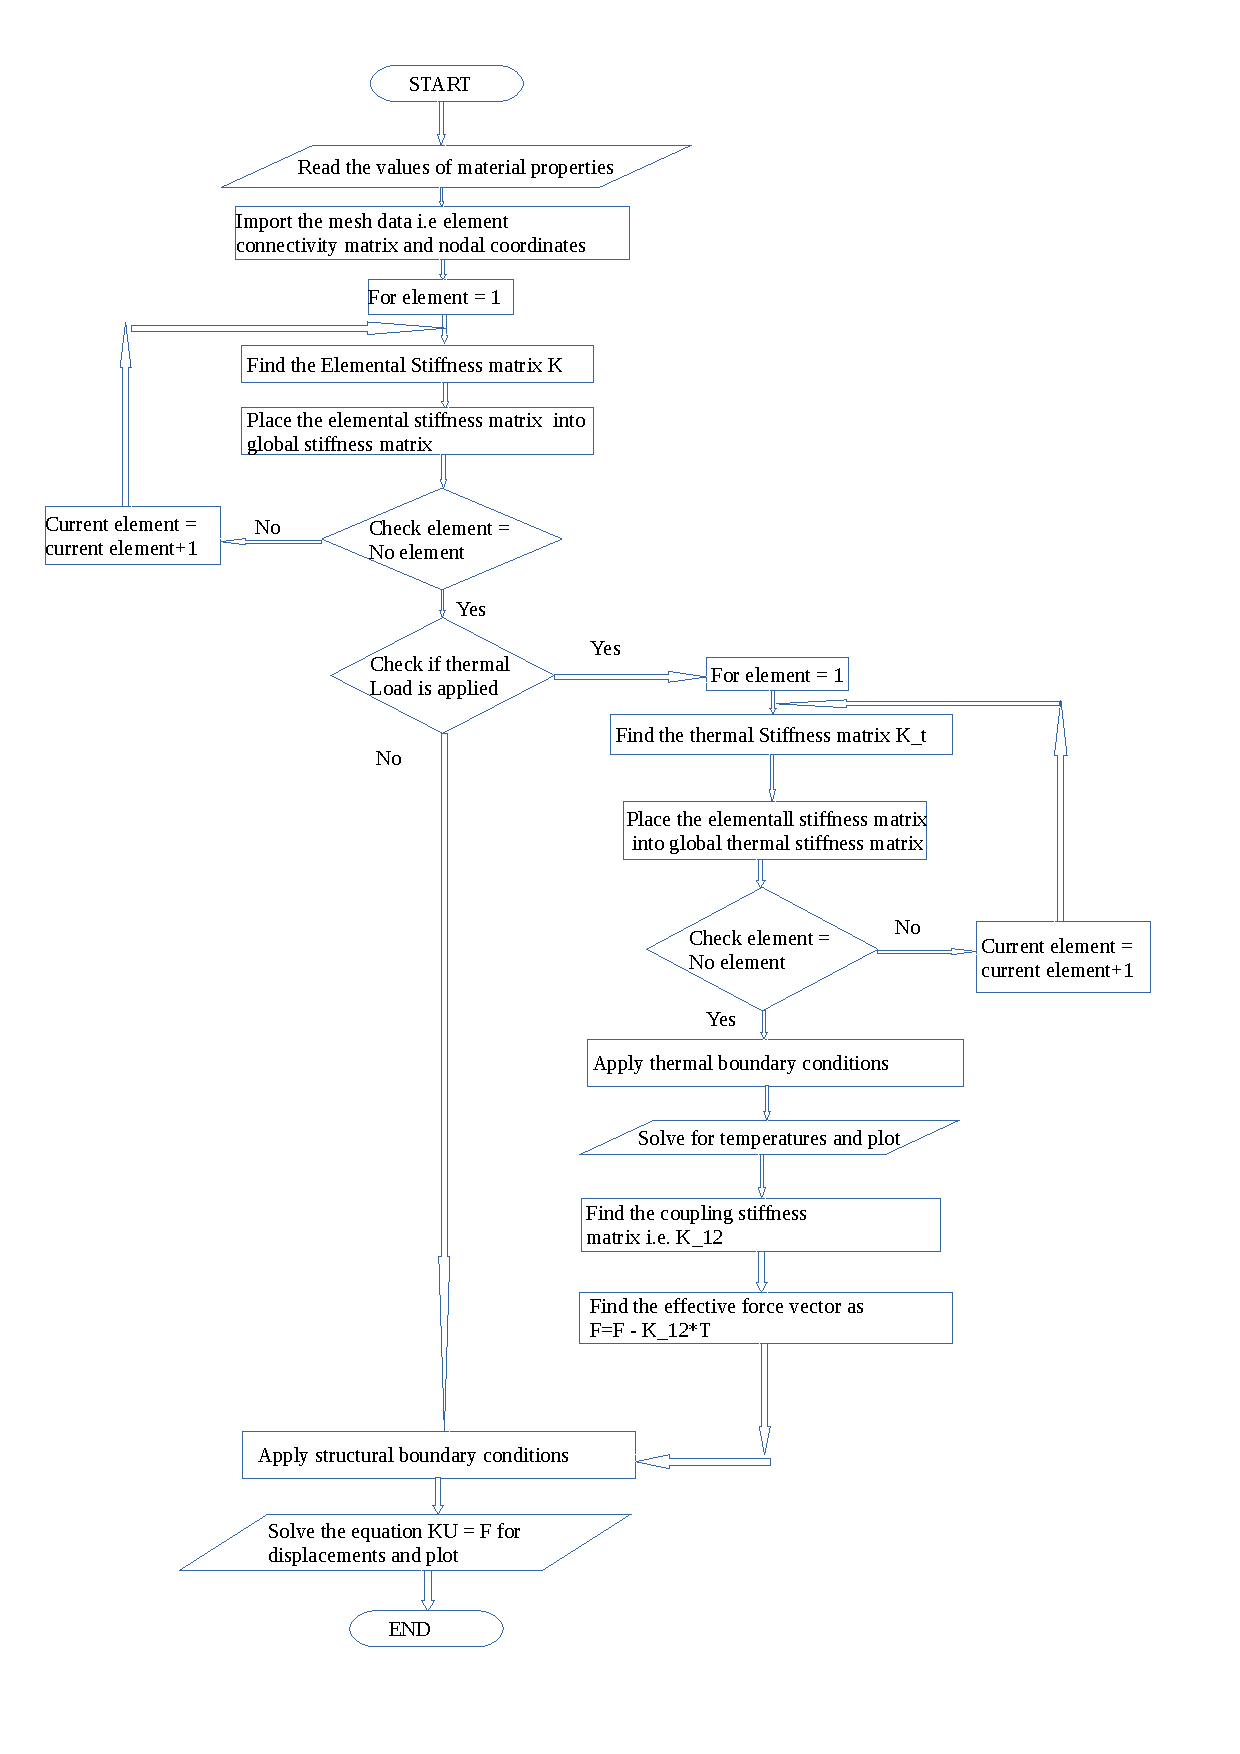
\includegraphics[width=0.48\textwidth]{flow_chart.pdf}
  \end{center}
\caption{Flowchart showing the steps of the FEM program}
\end{wrapfigure}
A MATLAB program is developed to solve the 2-dimensional thermoelasticity problems.\\ \vspace{5pt} 
Quadrilateral (Q4) elements were used for meshing the body. \\ \vspace{5pt}  $2\times 2$ Gauss quadrature rule is used for numerical integration.\\ \vspace{5pt} 
A flow-chart showing the steps of the programming is shown in the figure.

\end{frame}
%%%%%%%%%%%%%%%%%%%%%%%%%%%%%%%%%%%%%%%%%%%%%%%%%%%%%%%%%%%%%%%%%%%%%
\begin{frame}[t,fragile]{Patch Test 1}
    \vspace{-.4cm}
    \footnotesize
 \begin{itemize}
        \item A square plate is taken and meshed with 4 elements as shown in figure below. 
        \item Minimum number of essential boundary conditions is fixed to eliminate the rigid body motions
        \item Loads are applied such that there is constant state of stress in the body
        \item Numerical integration is performed using $2\times 2$ Gauss quadrature rule.
    \end{itemize}
    \begin{figure}
    \vspace{.5cm}
\begin{subfigure}{0.45\textwidth}
    \centering
    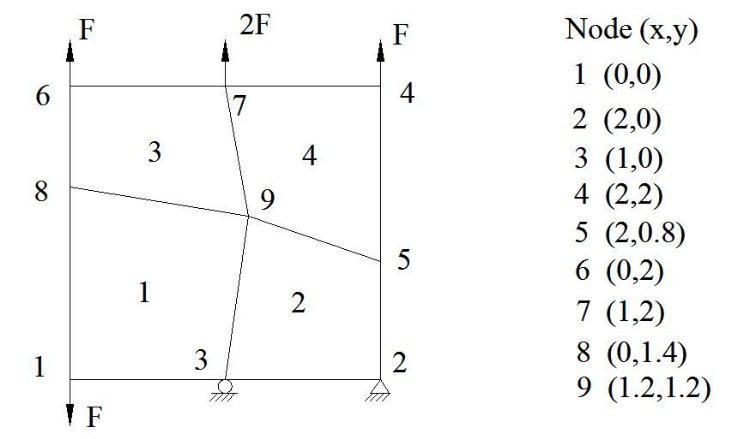
\includegraphics[scale=.25]{image1}
    \caption{\scriptsize Mesh Configuration }
\end{subfigure}
\begin{subfigure}{0.45\textwidth}
    \vspace{-.5cm}
    \centering
\caption{\scriptsize Results of Patch Test 1}
\scalebox{.5}{ \begin{tabular}{|c|c|c|c|c|}
\hline
& Gauss Points& $\sigma_x/2F$ & $\sigma_y/2F$ & $\tau_{xy}/2F$\\
\hline
\multirow{4}{5em}{Element 1} & 1 & $-0.222\times 10^{-15}$ & 1 & $0.1665\times 10^{-15}$\\
& 2 & $0.2498\times 10^{-15}$ & 1 & $0.1665\times 10^{-15}$\\
& 3 & $0.3058\times 10^{-15}$ & 1 & $0.222\times 10^{-15}$\\
& 4 & $0$ & 1 & $0$\\
\hline
\multirow{4}{5em}{Element 2} & 1 & $-0.222\times 10^{-15}$ & 1 & $0$\\
& 2 & $-.41633\times 10^{-15}$ & 1 & $0.111\times 10^{-15}$\\
& 3 & $0.02775\times 10^{-15}$ & 1 & $0.138\times 10^{-15}$\\
& 4 & $-0.1110\times 10^{-15}$ & 1 & $0$\\
\hline
\multirow{4}{5em}{Element 3} & 1 & $0.222\times 10^{-15}$ & 1 & $0.1665\times 10^{-15}$\\
& 2 & $0.0555\times 10^{-15}$ & 1 & $0.222\times 10^{-15}$\\
& 3 & $-0.0555\times 10^{-15}$ & 1 & $0$\\
& 4 & $0.22204\times 10^{-15}$ & 1 & $0$\\
\hline
\multirow{4}{5em}{Element 4} & 1 & $-0.222\times 10^{-15}$ & 1 & $0.1665\times 10^{-15}$\\
& 2 & $0.222\times 10^{-15}$ & 1 & $0.1665\times 10^{-15}$\\
& 3 & $0.3058\times 10^{-15}$ & 1 & $0.222\times 10^{-15}$\\
& 4 & $0.222\times 10^{-15}$ & 1 & $0$\\
\hline
\end{tabular}}
      \end{subfigure}
  \end{figure}
\end{frame}
%%%%%%%%%%%%%%%%%%%%%%%%%%%%%%%%%%%%%%%%%%%%%%%%%%%%%%%%%%%%%%%%%%%%%%%%%%%%
\begin{frame}[t,fragile]{Patch Test 2}
    \vspace{-.4cm}
    \footnotesize
 \begin{itemize}
        \item A square plate is taken and meshed with 4 elements as shown in figure below. 
        \item Minimum number of essential boundary conditions is fixed to eliminate the rigid body motions
        \item Loads are applied such that there is constant state of stress in the body
        \item Numerical integration is performed using $2\times 2$ Gauss quadrature rule.
    \end{itemize}
    \begin{figure}
    \vspace{.5cm}
\begin{subfigure}{0.45\textwidth}
    \centering
    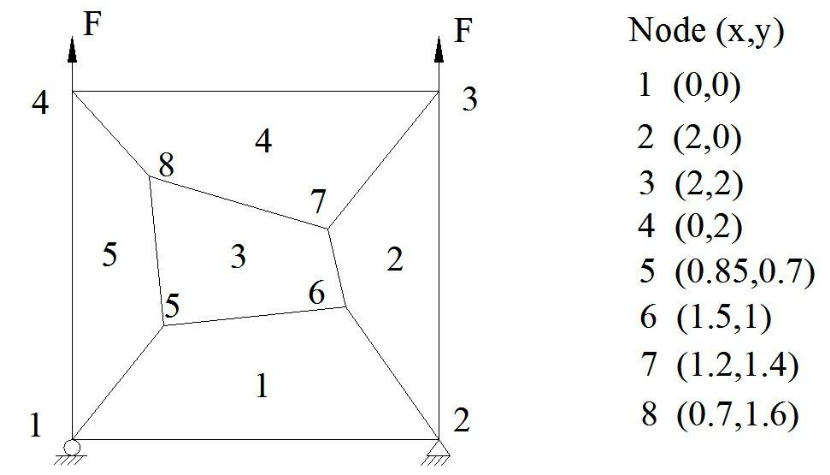
\includegraphics[scale=.2]{image2}
    \caption{\scriptsize Mesh Configuration }
\end{subfigure}
\begin{subfigure}{0.45\textwidth}
    \vspace{-.5cm}
     \centering
\caption{\scriptsize Results of Patch Test 2}
 \scalebox{.5}{\begin{tabular}{|c|c|c|c|c|}
\hline
& Gauss Point& $\sigma_x/F$ & $\sigma_y/F$ & $\tau_{xy}/F$\\
\hline
\multirow{4}{5em}{Element 1} & 1 & $0.166\times 10^{-15}$ &1& $0.1665\times 10^{-15}$\\
& 2 & $-0.033\times 10^{-15}$ &1& $0.1665\times 10^{-15}$\\
& 3 & $-0.063\times 10^{-15}$ &1& $0.222\times 10^{-15}$\\
& 4 & $0$ &1& $0$\\
\hline
\multirow{4}{5em}{Element 2} & 1 & $0.062\times 10^{-15}$ &1& $0$\\
& 2 & $-.41633\times 10^{-15}$ &1& $-0.222\times 10^{-15}$\\
& 3 & $0.02775\times 10^{-15}$ &1& $0.138\times 10^{-15}$\\
& 4 & $-0.2220\times 10^{-15}$ &1& $0$\\
\hline
\multirow{4}{5em}{Element 3} & 1 & $0.222\times 10^{-15}$ &1& $0.1665\times 10^{-15}$\\
& 2 & $0.0555\times 10^{-15}$ &1& $0.222\times 10^{-15}$\\
& 3 & $-0.0555\times 10^{-15}$ &1& $0$\\
& 4 & $0.22204\times 10^{-15}$ &1& $0$\\
\hline
\multirow{4}{5em}{Element 4} & 1 & $-0.222\times 10^{-15}$ &1& $0.1665\times 10^{-15}$\\
& 2 & $0.222\times 10^{-15}$ &1& $0.1665\times 10^{-15}$\\
& 3 & $-0.063\times 10^{-15}$ &1& $0.222\times 10^{-15}$\\
& 4 & $0.222\times 10^{-15}$ &1& $0$\\
\hline
\multirow{4}{5em}{Element 5} & 1 & $-0.422\times 10^{-15}$ &1& $0.1665\times 10^{-15}$\\
& 2 & $0.222\times 10^{-15}$ &1& $0.1665\times 10^{-15}$\\
& 3 & $-0.063\times 10^{-15}$ &1& $0.222\times 10^{-15}$\\
& 4 & $0.222\times 10^{-15}$ &1& $0$\\
\hline
\end{tabular}}
     \end{subfigure}
  \end{figure}
\end{frame}
%%%%%%%%%%%%%%%%%%%%%%%%%%%%%%%%%%%%%%%%%%%%%%%%%%%%%%%%%%%%%%%%%%%%%%%%%%%%
\begin{frame}[t,fragile]{Patch Test for thermal code }
    \vspace{-.4cm}
    \footnotesize
 \begin{itemize}
        \item A square plate is taken and meshed with 4 elements as shown in figure below. 
        \item Minimum number of essential boundary conditions is fixed to eliminate the rigid body motions
        \item Loads are applied such that there is constant state of stress in the body
        \item Numerical integration is performed using $2\times 2$ Gauss quadrature rule.
    \end{itemize}
    \begin{figure}
    \vspace{.5cm}
    \hspace{-.5cm}
\begin{subfigure}{0.3\textwidth}
     \centering
    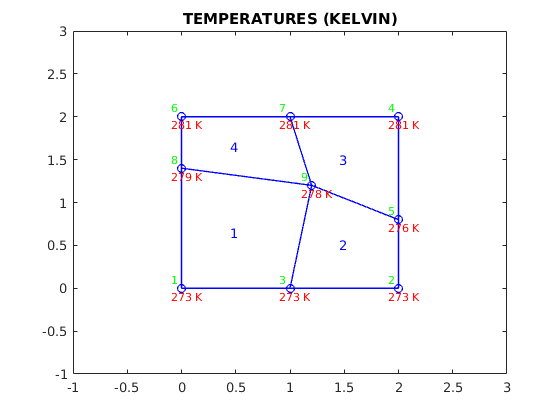
\includegraphics[scale=.2]{solution.jpg}
    \caption{\tiny Temperature distribution}
\end{subfigure}
\begin{subfigure}{0.6\textwidth}
    \vspace{-1cm}
    \centering
    \caption{\scriptsize Results of Patch test 3}
 \scalebox{.55}{\begin{tabular}{|C{3cm}|C{3cm}|C{3cm}|C{3cm}|}
        \hline
        Nodes&Temperatures&$Q_y(W)$&$Q_x(W)$\\
        \hline
        1&273&200&$0.125\times 10^{-10}$\\
        \hline
        2&273&200&$0.155\times 10^{-10}$\\
        \hline
        3&273&200&$0.222\times 10^{-10}$\\
        \hline
        4&281&200&0\\
        \hline
        5&276&200&$0$\\
        \hline
        6&281&200&$0$\\
        \hline
        7&281&200&$0.111\times 10^{-10}$\\
        \hline
        8&279&200&$0.138\times 10^{-10}$\\
        \hline
        9&278&200&$0$\\
        \hline
    \end{tabular}}
     \end{subfigure}
  \end{figure}
\end{frame}
%%%%%%%%%%%%%%%%%%%%%%%%%%%%%%%%%%%%%%%%%%%%%%%%%%%%%%%%%%%%%%%%%%%%%%%%%
\begin{frame}[t,fragile]{Patch Test for Thermo-elastic code: Poisson's equation}
\begin{figure}[H]
    \centering
    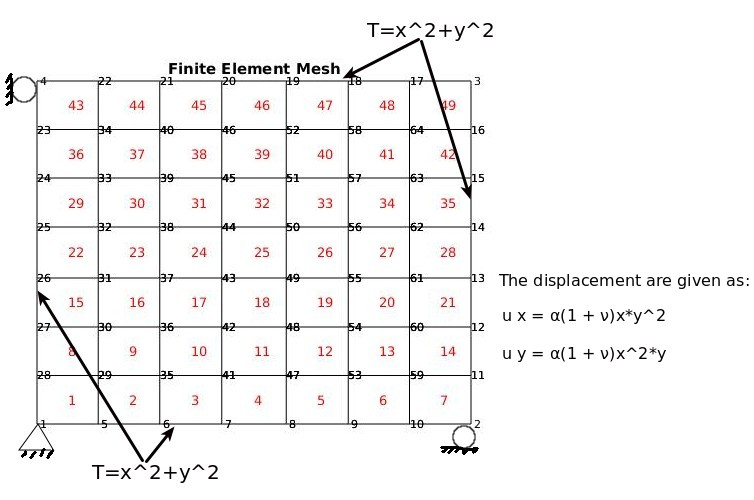
\includegraphics[scale=.4]{elements_7^2_1.jpg}
    \caption{mesh configuration of plate}
    \label{thfig1}
\end{figure}

\end{frame}
%%%%%%%%%%%%%%%%%%%%%%%%%%%%%%%%%%%%%%%%%%%%%%%%%%%%%%%%%%%%%%%%%%%%%%% 
\begin{frame}[t,fragile]{Mesh Refinements}
    \begin{figure}
    \centering
\begin{tikzpicture}[      
        every node/.style={scale=.6,anchor=south west,inner sep=0pt},
        x=1mm, y=1mm,scale=.6
      ] 
       \node (fig2) at (-25,-35)
       {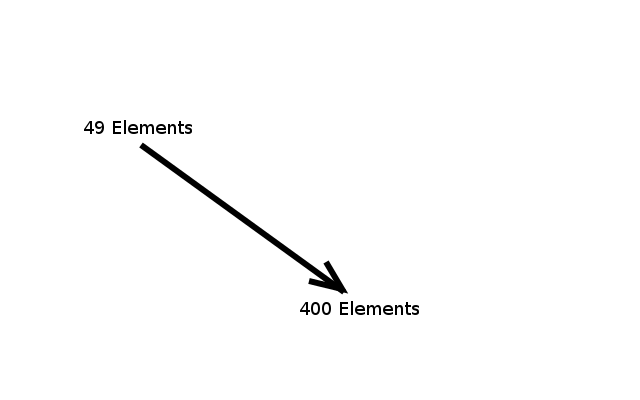
\includegraphics[scale=0.35]{arrow}};  
     \node (fig1) at (0,0)
       {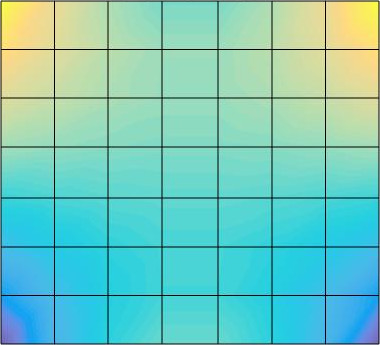
\includegraphics[scale=0.3]{uy_7^2}};
    \node (fig2) at (10,-10)
       {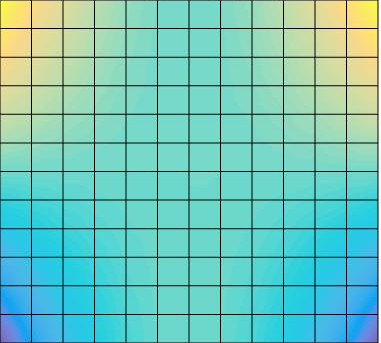
\includegraphics[scale=0.3]{uy_12^2}};
     \node (fig2) at (20,-20)
       {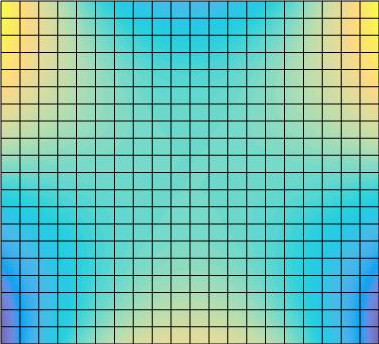
\includegraphics[scale=0.3]{uy_20^2}};  
    \end{tikzpicture}
\end{figure}
\vspace{-1cm}
\begin{figure}
   \centering
    \caption{\scriptsize Errors obtained after mesh refinements }
    \vspace{-16pt}
 \scalebox{.6}{\begin{tabular}{|c|c|c|c|c|c|}
        \hline
       Number of Elements & Error in  $u_x$ & Error in  $u_y$ & Error in  $\sigma_x$ & Error in  $\sigma_y$ & Error in  $\tau_{xy}$\\
        \hline
       $7\times 7$ & $5.783469\times 10^{-10}$ & $5.783469\times 10^{-10}$ & $6.668255\times 10^{2}$ & $6.668255\times 10^{2}$ & $3.615391\times 10^{2}$\\
        \hline
         $12\times 12$ & $1.764697\times 10^{-11}$ & $1.764697\times 10^{-11}$ & $1.000597121$ & $1.000597121$ & $0.031722$\\
        \hline
        $20\times 20$ & $1.265804\times 10^{-12}$ & $1.265804\times 10^{-12}$ & $0.994299467$ & $0.994299467$ & $0.005781$\\
        \hline
    \end{tabular}}
\end{figure}
\end{frame}
%%%%%%%%%%%%%%%%%%%%%%%%%%%%%%%%%%%%%%%%%%%%%%%%%%%%%%%%%%%%%%%%%%%%%%%%%
\begin{frame}[t,fragile]{Plate with edge crack}
    \vspace{-.4cm}
   \begin{figure}[H]
    \centering
        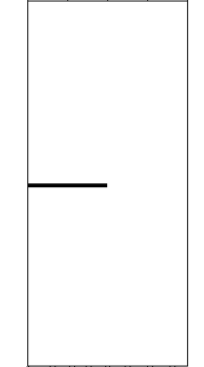
\includegraphics[scale=.15]{1.png}
        \vspace{-10pt}
        \caption{\tiny Plate with edge crack}
    \end{figure}
        \vspace{-16pt}
    \begin{figure}
    \begin{subfigure}{.3\textwidth}
         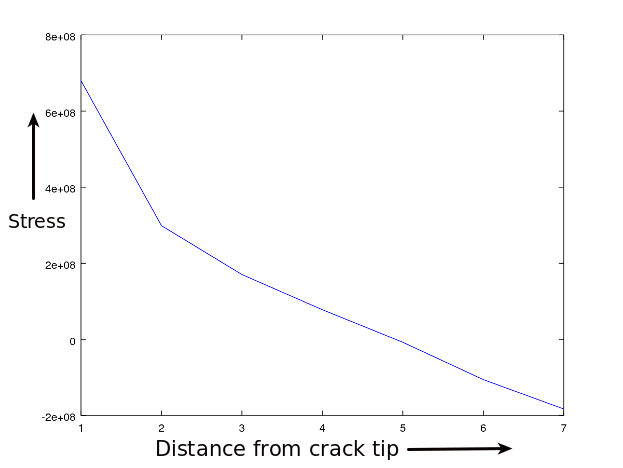
\includegraphics[scale=.2]{onlystress}
    \caption{\tiny $\sigma_y$ ahead of the crack tip}
    \label{stress}
\end{subfigure}
\hspace{1pt}
    \begin{subfigure}{.3\textwidth}
    \centering
    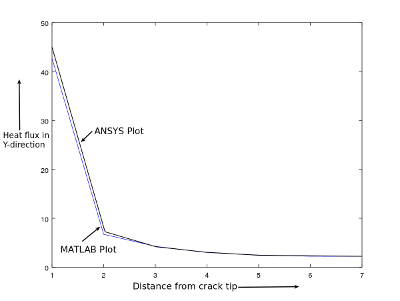
\includegraphics[scale=.2]{onlytempqy}
    \caption{\tiny Heat flux ahead of crack tip}
    \label{fig:heat}
\end{subfigure}
\hspace{1pt}
    \begin{subfigure}{.3\textwidth}
        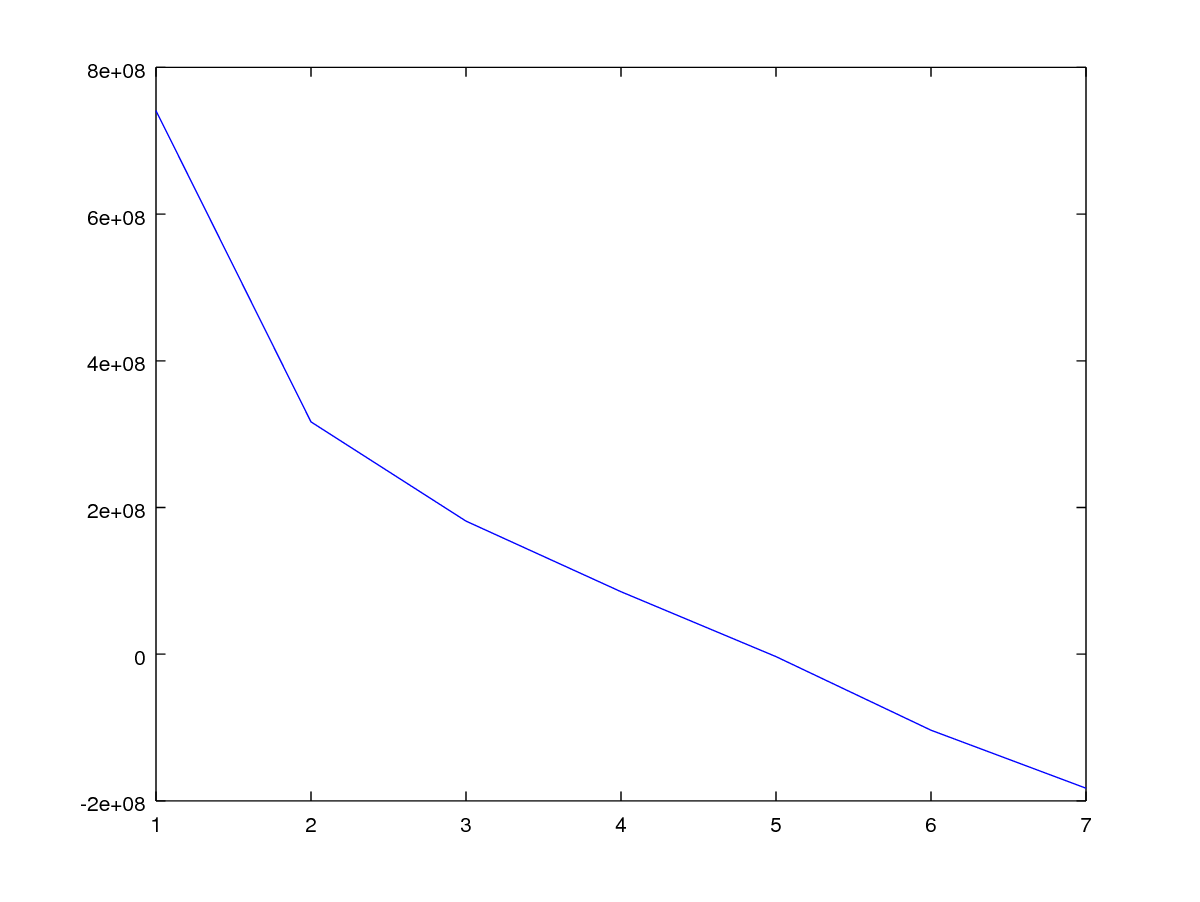
\includegraphics[scale=.2]{only_bothstress}
        \caption{\tiny $\sigma_y$ ahead of the crack tip}
    \label{heat1}
\end{subfigure}
\end{figure}
\end{frame}
%%%%%%%%%%%%%%%%%%%%%%%%%%%%%%%%%%%%%%%%%%%%%%%%%%%%%%%%%%%%%%%5
\end{document}
